\chapter{System Interaction Diagrams}

% This chapter requires a good 1-2 pages
% prefacing the way systems will behave
% and introducing the types of diagrams
% that will be shown.

\section{Introduction}

The interaction diagrams in the following section will outline the system
interactions in the most important parts of our software. For each particular
use case, we will outline the interactions among the systems and databases.
Further, we will analyze multiple cases in which the systems will handle
different scenarios. That is, it will show how the system handles both failure
and success conditions. In the following scenarios, you will see the database,
controller, and Yahoo! Finance API used in nearly every situation. Because this
is a web-based and data based application, the database and controller become
heavily prevalent. Users will need to log in and constantly access data pulled
from the Yahoo! Finance API to have constantly refreshed and updated
information. The diagrams below will accurately detail how this will be
accomplished within the system.

\section{Diagrams}

\subsection{Use Case 1}

Shown in the sequence diagram for UC-1 begins with two options for the Guest.
Either login or register an account. If a user attempts to register a new
account the Account Controller is contacted with the user’s information. Then
the Account Controller can attempt to check to make sure no duplicate login
information exists in the database via the DB Connection module and if not it
will store the new user information into the database. After this happens the
user will be sent a confirmation email. Then the Account Controller will update
the Login View.\\

If a user attempts to login, the Account Controller will attempt to authenticate
the login details with details found in the database via the DB Connection
module. If the details match correctly then the Account Controller will send the
guest into investor mode and therefore displaying them the Player Profile View.

\begin{figure}[H]
\centering
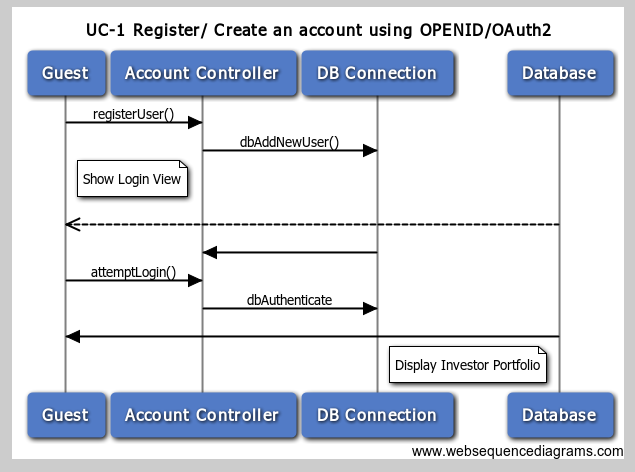
\includegraphics[width=5.5in]{./img/inter/UC1.png}
\caption{UC-1}
\end{figure}

\subsection{Use Case 2}
Shown in the sequence diagram for UC-2 is the flow of how to create an
investment league. When an investor selects to create a league the League
Controller will be contacted. This will update the Player Profile View display
the available options for creating a league. After, there is a function
updateSettings() which will create the league and process it in the database
via the DB Connection and also allow settings to be updated for a league. Not
shown in the diagram is the alternative case of joining a league. The process
to join a league is straightforward, where the league controller will show
available leagues and then if an investor chooses to join they will be entered
into the list in the database to associate with this league.

\begin{figure}[H]
\centering
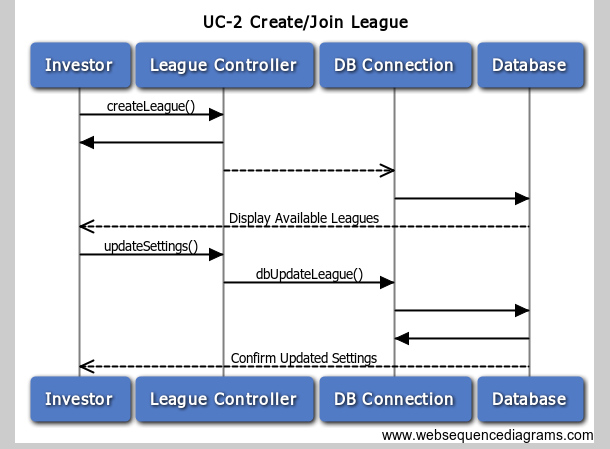
\includegraphics[width=5.5in]{./img/inter/UC2.png}
\caption{UC-2}
\end{figure}

\subsection{Use Case 3}
Viewing market data is accomplished by an investor searching a term. The Order
System Controller then finds this term which is most likely a company name or
stock symbol. The system will fetch matches from the database via the DB
Connection module and display them from the user. The investor will choose a
match. The Order System Controller takes the chosen term and requests its data
from the Yahoo! Finance API via the Yahoo! Finance Adapter. The Order System
Controller will update the database via the DB Connection module for this term,
and then continue to show the Market Data View.\\


\begin{figure}[H]
\centering
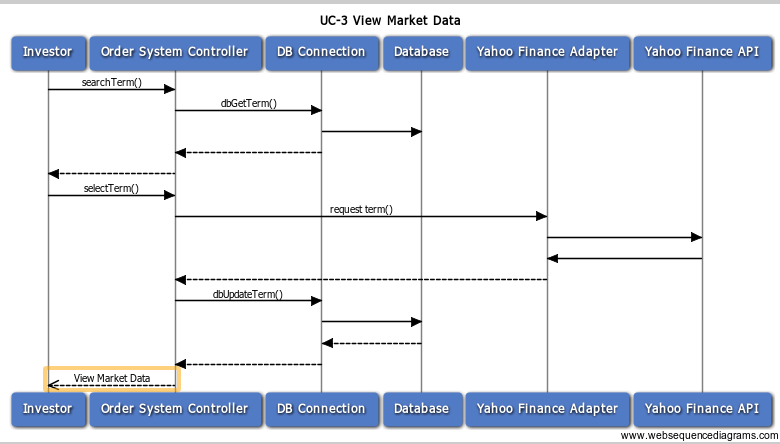
\includegraphics[width=5.5in]{./img/inter/UC3.png}
\caption{UC-3}
\end{figure}

\subsection{Use Case 4}
The investor should be able to view and make changes to their Portfolio View.
When the user clicks to show portfolio, the Portfolio Controller will fetch the
investor’s portfolio stocks from the database via the DB Connection module. The
investor can also update their view of the portfolio and other settings.

\begin{figure}[H]
\centering
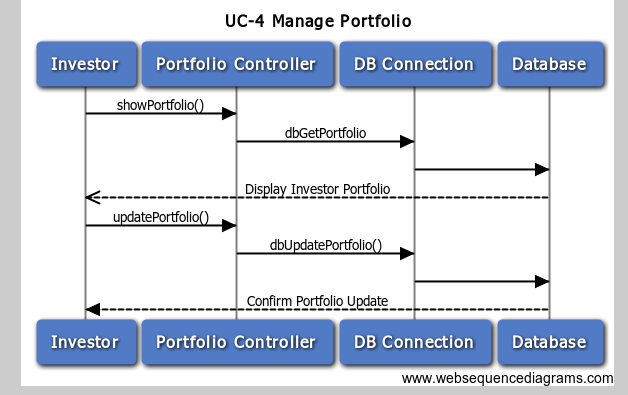
\includegraphics[width=5.5in]{./img/inter/UC4.png}
\caption{UC-4}
\end{figure}

\subsection{Use Case 5}
The investor needs to be able to place market orders. As soon as the investor
places an order the Order System Controller contacts Yahoo! Finance API via the
Yahoo! Finance Adapter to retrieve the current price of the stock. After the
current price is found the Order System Controller must confirm with the
database via the DB Connection module that the user has enough funds to make a
buy order or enough stock to make the sell order. After the trade is confirmed
information will be stored about it in the database via the DB Connection
module and the changes will be displayed in the investor’s portfolio.

\begin{figure}[H]
\centering
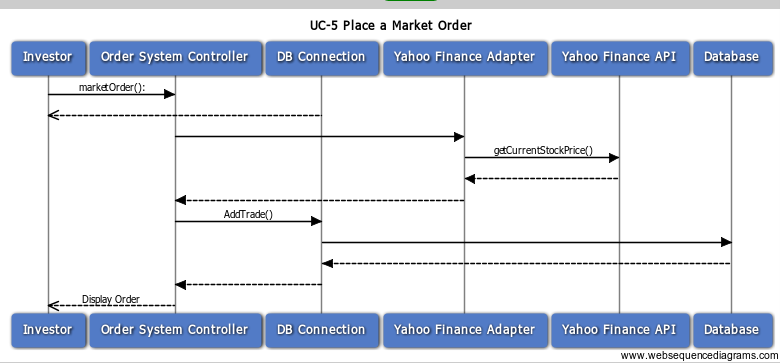
\includegraphics[width=5.5in]{./img/inter/UC5.png}
\caption{UC-5}
\end{figure}

\subsection{Pub/Sub for Achievements}
We decided to us a Publisher/Subscribe pattern to handle achievements on the
server, and use that to update the user interface and database.  This will
allow us to handle all the achievement handling in one location, instead of
spreading the logic throughout the code.  This will greatly ease our ability
to introduce additional achievements as the application matures, as well as
easily fix bugs in our achievement handling system.

\begin{figure}[H]
\centering
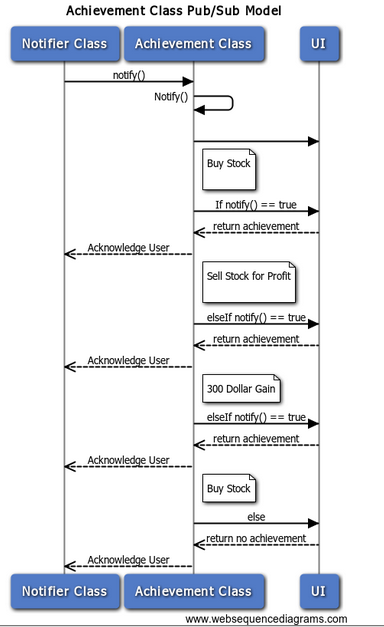
\includegraphics[width=5.5in]{./img/inter/PubSub.png}
\caption{UC-5}
\end{figure}


\section{Alternate Solution Diagramming}

Software design shouldn't be about picking your first idea and going with it.
You need to consider alternative solutions to the task at hand and pick the best
one based on the known criteria.  For this reason we are documenting some of
our alternative solutions for historical reference.\\

\begin{figure}[H]
\centering
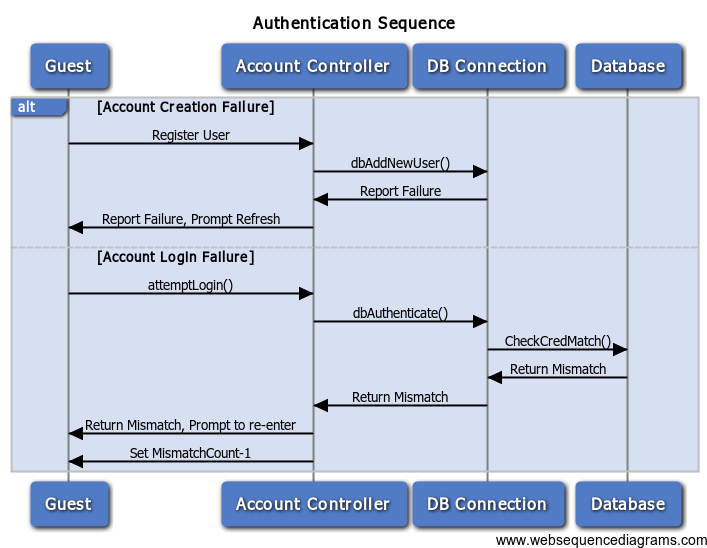
\includegraphics[width=5.5in]{./img/inter/alt1.png}
\caption{UC-1 alternate solution considered}
\end{figure}
\begin{figure}[H]
\centering
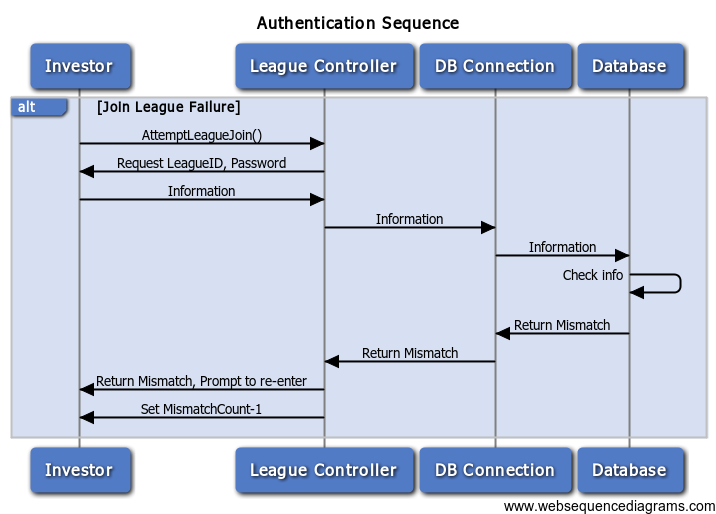
\includegraphics[width=5.5in]{./img/inter/alt2.png}
\caption{UC-2 alternate solution considered}
\end{figure}
\begin{figure}[H]
\centering
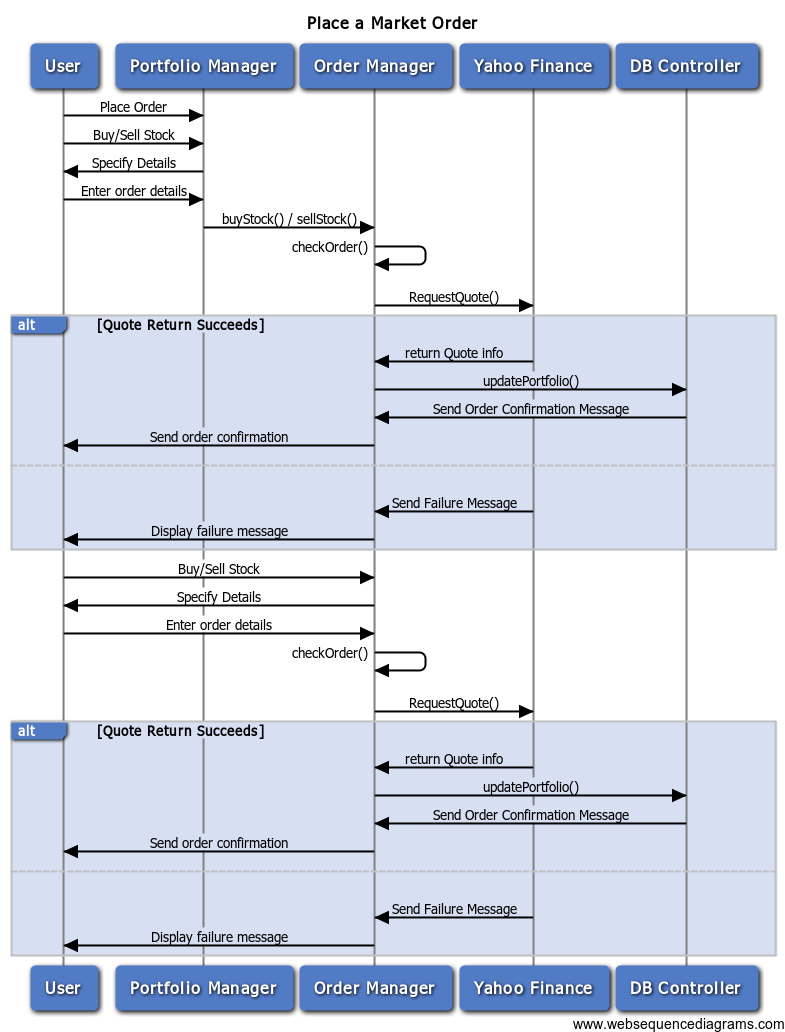
\includegraphics[width=5.5in]{./img/inter/alt3.png}
\caption{UC-3 alternate solution considered}
\end{figure}
\begin{figure}[H]
\centering
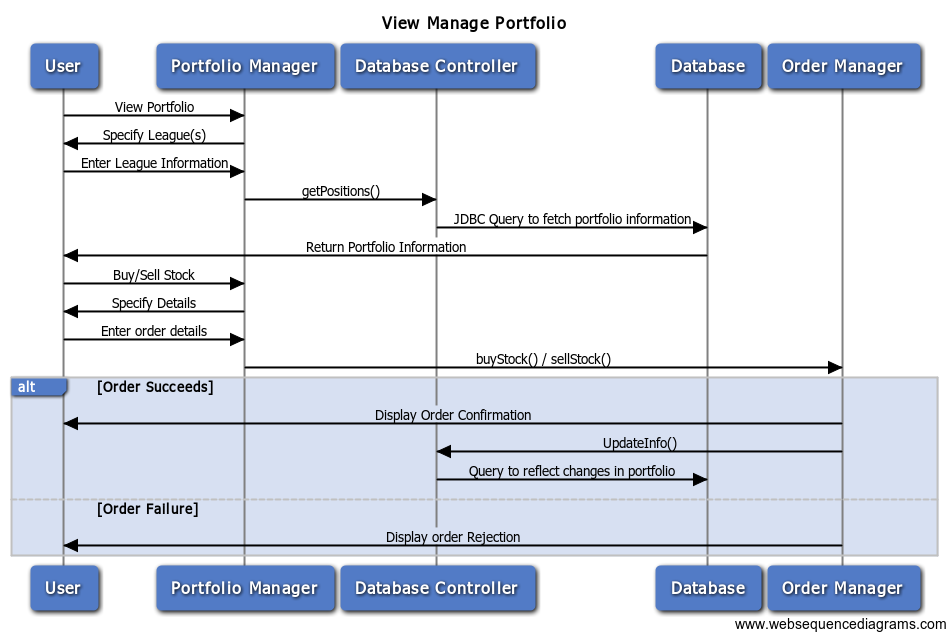
\includegraphics[width=5.5in]{./img/inter/alt4.png}
\caption{UC-4 alternate solution considered}
\end{figure}
\begin{figure}[H]
\centering
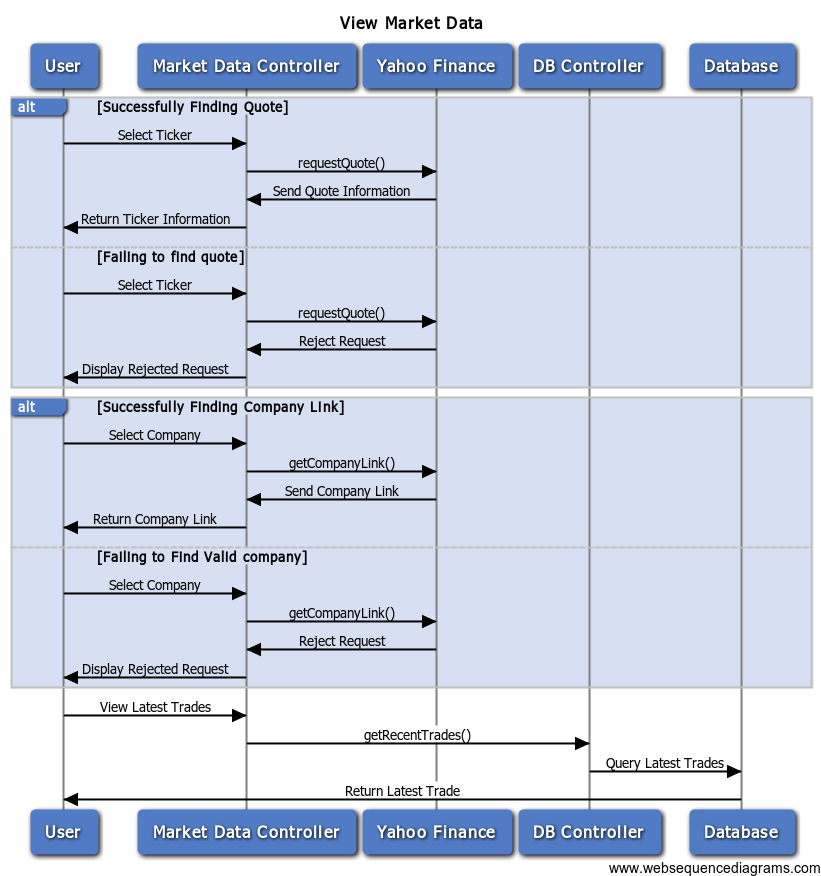
\includegraphics[width=5.5in]{./img/inter/alt5.png}
\caption{UC-5 alternate solution considered}
\end{figure}

\section{Design Patterns}

\section{Design Patterns}
Various standard and non-standard design patterns were utilized to provide
functionality for things such as authentication, efficient page rendering and
object modeling.

\subsection{Model-View-Controller}
The Model-View-Controller (MVC) pattern was heavily used throughout the system
to properly organize model logic, business logic and presentation logic. This
very intuitive pattern allowed the team to easily delegate work on different
levels of the system. Frequently, a selection of team members would develop
front-end functionality which required only the views to be altered, while other
members implemented backend functionality which was done either in controllers
or models. This pattern resulted in a more efficient development lifecycle
overall, while also providing some performance gains. Namely, the MVC pattern
calls on resources only when they are actually needed which prevents unnecessary
overhead. For example, methods developed to be called only programmatically
don't attempt to display a view which results in faster responses.
\subsection{Publisher Subscribe}
The Publisher/Subscribe pattern allows us to easily decouple our handling of
business logic from that of our game logic, most notably, our achievements
system. This allows us to easily change business logic without having to read
through code dedicated to achievement handling. More importantly, it allows us
to be able to easily add, update, and delete achievement handling code within the
confines of a single class. We also believe that we can use the
Publish/Subscribe model in the future to extend functionality to limit and stop
orders, allowing actors to be updated once an order has been completed.
\subsection{Object Relational Model Pattern}
The Object Relational Model (ORM) pattern, an intelligent implementation of a
database access design pattern, was used exclusively to interact with
persistent storage technologies used in the system. This pattern offered the
major advantage of not needing to hard code any database-specific queries. All
requests made through the ORM are translated to the currently used DB system's
language and data is returned in directly its object form. The lack of need to
write direct queries also lead to a great side effect, namely database
agnosticism which allowed various database implementations to be tested during
different stages of development. During development SQLite was used for its
lightweight footprint on the developers machine, then for production MySQL was
used as it is considerably more efficient when dealing with larger amounts of
data. This design certainly improved our development by saving countless hours
of development time.
\subsection{RESTful Design}
The RESTful design pattern being used more and more now on the web allowed us to
implement our asynchronous order processing system. The RESTful design of some
internal functionality allowed it to be accessed programmatically and securely
through a simple API. As RESTful services are at the heart of the Play
Framework, it did not require a lot of effort to expose some internal
functionality without creating major security holes. Future iterations will
continue to rely on the stateful communication that our RESTful API offers.
\subsection{Responsive UI Pattern}
The Bootstrap UI framework implemented a design pattern completely segregating
visual presentation from content and user experience. This provided a beautiful
responsive design which adapted to different client devices ranging from
desktops to smart devices. The pattern takes advantage of the flexible markup of
HTML5 to customize it on the fly when the page is rendering in the browser using
Javascript and CSS. This allowed our team to target the rapidly growing mobile
users without much extra implementation effort. It also inherently produced a
faster user experience since minimal processing is done during initial page
rendering and mostly done asynchronously once the page is already viewable to
the user. We actively strived to achieve both of these goals.
